\documentclass[a4paper, 12pt]{article}

% ~~~~~~~~~~~~~~~~~~~~~~~~~~~~~~~~~~~~~~~~
% ~~~~~~~~~~~~~~~ PACKAGES ~~~~~~~~~~~~~~~
% ~~~~~~~~~~~~~~~~~~~~~~~~~~~~~~~~~~~~~~~~

\usepackage{amsmath}
\usepackage{relsize}
\usepackage{tikz}
\usepackage{xcolor}

% ~~~~~~~~~~~~~~~~~~~~~~~~~~~~~~~~~~~~~~~~
% ~~~~~~~~~~~~~~~ PREAMBLE ~~~~~~~~~~~~~~~
% ~~~~~~~~~~~~~~~~~~~~~~~~~~~~~~~~~~~~~~~~

\title{Demo Document No. 1\\[0.4em]\smaller{for the SEPTeX module}}
\author{Marcel Simader}
\pagenumbering{gobble}
% This is indeed a comment in the preamble

% ~~~~~~~~~~~~~~~~~~~~~~~~~~~~~~~~~~~~
% ~~~~~~~~~~~~~~~ BODY ~~~~~~~~~~~~~~~
% ~~~~~~~~~~~~~~~~~~~~~~~~~~~~~~~~~~~~

\begin{document}
	\maketitle
	
	\noindent This is some text, and it contains a potentially % confusing comment for the "soft" line wrap % functionality
	
	And this is some text that goes on and on and on and on and on and on and on and on and on and on and on and on and on and
 on and on and on and on and on and on and on and on\ldots
	This is a \LaTeX\ sentence -- wow!
	\begin{gather*}
		\left[ 1, \frac{1}{3}, 3, \text{abc} \right]
		\left\{ abc, 1, -\frac{2}{7}, -\frac{3}{5} \right\}
		\\
		\left( \left\{ 1, 2, 3, -\frac{9}{2} \right\}, \text{addition} \right)
		\left( \left\{ 1, 2, 3, -\frac{9}{2} \right\}, \text{addition}, \text{addition} \right)
	\end{gather*}
	
	\newpage
	
	\begin{figure}[h!]
		\begin{center}
			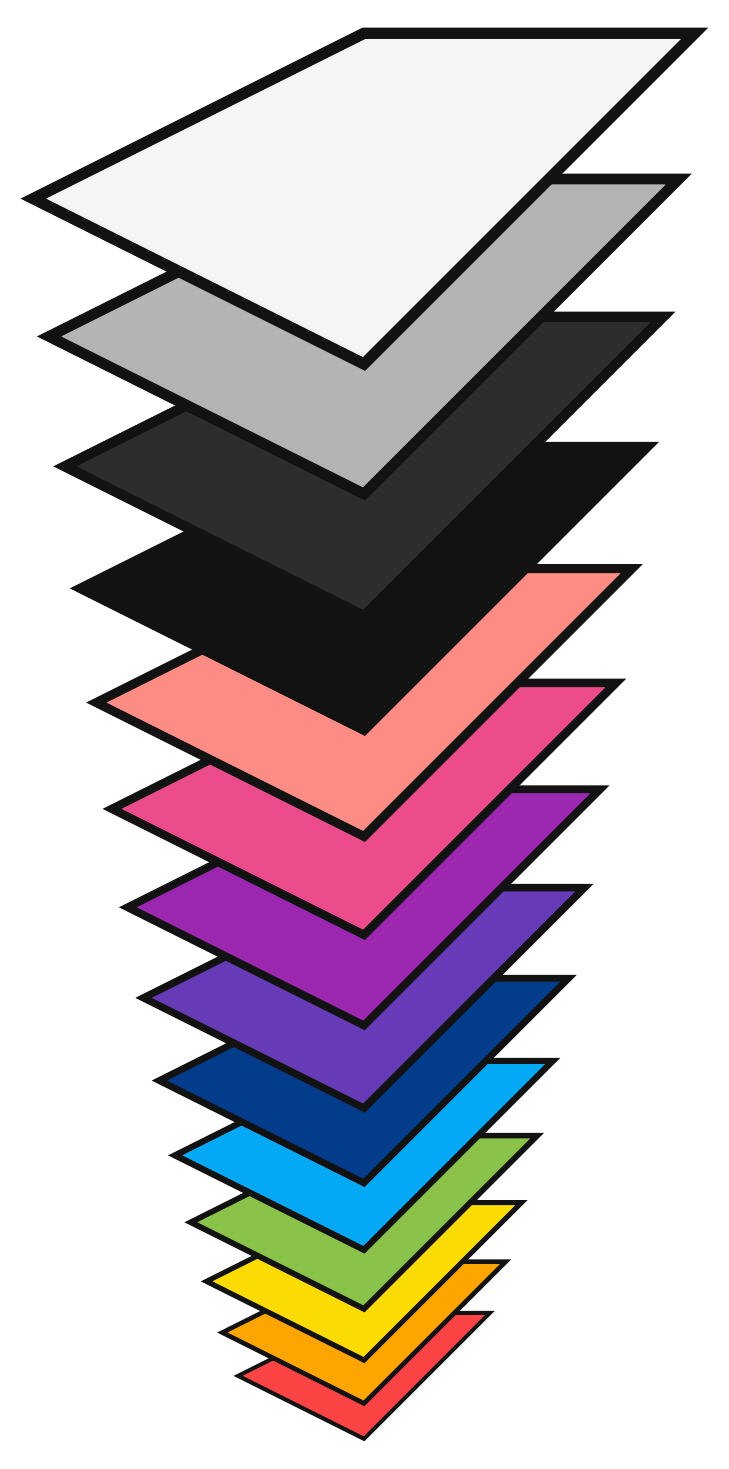
\begin{tikzpicture}
				\definecolor{RED}{RGB}{252, 68, 68}
				\definecolor{ORANGE}{RGB}{255, 165, 0}
				\definecolor{YELLOW}{RGB}{251, 219, 4}
				\definecolor{GREEN}{RGB}{139, 195, 74}
				\definecolor{LIGHT_BLUE}{RGB}{3, 169, 244}
				\definecolor{DARK_BLUE}{RGB}{4, 60, 140}
				\definecolor{PURPLE}{RGB}{103, 58, 183}
				\definecolor{MAGENTA}{RGB}{156, 39, 176}
				\definecolor{PINK}{RGB}{236, 76, 140}
				\definecolor{ROSE}{RGB}{252, 140, 132}
				\definecolor{ALMOST_BLACK}{RGB}{18, 18, 18}
				\definecolor{DARK_GRAY}{RGB}{45, 45, 45}
				\definecolor{LIGHT_GRAY}{RGB}{180, 180, 180}
				\definecolor{ALMOST_WHITE}{RGB}{245, 245, 245}
				\begin{scope}[scale={0.4}]
					\draw[line width={0.5mm}, color={ALMOST_BLACK}, fill={RED}] (0.00cm, 0.00cm) -- (4.00cm, 4.00cm) -- (0.00cm, 4.00cm)
 -- (-4.00cm, 2.00cm) -- cycle;
				\end{scope}
				
				\begin{scope}[scale={0.45}]
					\draw[line width={0.5714285714285714mm}, color={ALMOST_BLACK}, fill={ORANGE}] (0.00cm, 1.00cm) -- (4.00cm, 5.00cm) --
 (0.00cm, 5.00cm) -- (-4.00cm, 3.00cm) -- cycle;
				\end{scope}
				
				\begin{scope}[scale={0.5}]
					\draw[line width={0.6428571428571428mm}, color={ALMOST_BLACK}, fill={YELLOW}] (0.00cm, 2.00cm) -- (4.00cm, 6.00cm) --
 (0.00cm, 6.00cm) -- (-4.00cm, 4.00cm) -- cycle;
				\end{scope}
				
				\begin{scope}[scale={0.55}]
					\draw[line width={0.7142857142857143mm}, color={ALMOST_BLACK}, fill={GREEN}] (0.00cm, 3.00cm) -- (4.00cm, 7.00cm) --
 (0.00cm, 7.00cm) -- (-4.00cm, 5.00cm) -- cycle;
				\end{scope}
				
				\begin{scope}[scale={0.6}]
					\draw[line width={0.7857142857142857mm}, color={ALMOST_BLACK}, fill={LIGHT_BLUE}] (0.00cm, 4.00cm) -- (4.00cm, 8.00cm)
 -- (0.00cm, 8.00cm) -- (-4.00cm, 6.00cm) -- cycle;
				\end{scope}
				
				\begin{scope}[scale={0.65}]
					\draw[line width={0.8571428571428572mm}, color={ALMOST_BLACK}, fill={DARK_BLUE}] (0.00cm, 5.00cm) -- (4.00cm, 9.00cm)
 -- (0.00cm, 9.00cm) -- (-4.00cm, 7.00cm) -- cycle;
				\end{scope}
				
				\begin{scope}[scale={0.7}]
					\draw[line width={0.9285714285714286mm}, color={ALMOST_BLACK}, fill={PURPLE}] (0.00cm, 6.00cm) -- (4.00cm, 10.00cm)
 -- (0.00cm, 10.00cm) -- (-4.00cm, 8.00cm) -- cycle;
				\end{scope}
				
				\begin{scope}[scale={0.75}]
					\draw[line width={1.0mm}, color={ALMOST_BLACK}, fill={MAGENTA}] (0.00cm, 7.00cm) -- (4.00cm, 11.00cm) -- (0.00cm, 11.00cm)
 -- (-4.00cm, 9.00cm) -- cycle;
				\end{scope}
				
				\begin{scope}[scale={0.8}]
					\draw[line width={1.0714285714285714mm}, color={ALMOST_BLACK}, fill={PINK}] (0.00cm, 8.00cm) -- (4.00cm, 12.00cm) --
 (0.00cm, 12.00cm) -- (-4.00cm, 10.00cm) -- cycle;
				\end{scope}
				
				\begin{scope}[scale={0.8500000000000001}]
					\draw[line width={1.1428571428571428mm}, color={ALMOST_BLACK}, fill={ROSE}] (0.00cm, 9.00cm) -- (4.00cm, 13.00cm) --
 (0.00cm, 13.00cm) -- (-4.00cm, 11.00cm) -- cycle;
				\end{scope}
				
				\begin{scope}[scale={0.9}]
					\draw[line width={1.2142857142857144mm}, color={ALMOST_BLACK}, fill={ALMOST_BLACK}] (0.00cm, 10.00cm) -- (4.00cm, 14.00cm)
 -- (0.00cm, 14.00cm) -- (-4.00cm, 12.00cm) -- cycle;
				\end{scope}
				
				\begin{scope}[scale={0.95}]
					\draw[line width={1.2857142857142856mm}, color={ALMOST_BLACK}, fill={DARK_GRAY}] (0.00cm, 11.00cm) -- (4.00cm, 15.00cm)
 -- (0.00cm, 15.00cm) -- (-4.00cm, 13.00cm) -- cycle;
				\end{scope}
				
				\begin{scope}[scale={1.0}]
					\draw[line width={1.3571428571428572mm}, color={ALMOST_BLACK}, fill={LIGHT_GRAY}] (0.00cm, 12.00cm) -- (4.00cm, 16.00cm)
 -- (0.00cm, 16.00cm) -- (-4.00cm, 14.00cm) -- cycle;
				\end{scope}
				
				\begin{scope}[scale={1.05}]
					\draw[line width={1.4285714285714286mm}, color={ALMOST_BLACK}, fill={ALMOST_WHITE}] (0.00cm, 13.00cm) -- (4.00cm, 17.00cm)
 -- (0.00cm, 17.00cm) -- (-4.00cm, 15.00cm) -- cycle;
				\end{scope}
				
			\end{tikzpicture}
			
		\end{center}
		
		\caption{Captions, Figures, and the Default Colors.}
		\label{fig:}
	\end{figure}
	
\end{document}